\section{Data}\label{sec:data}
\paragraph{Dermoscopy} \emph{Controlled cohort:} ISIC 2018 Task 1/2 images with manual lesion masks and melanoma labels
(ISIC 2016/2017 tables); 2,437 images on which a $65\times19$\,px ruler can be placed at 0/25/50/75/100\% overlap with
the lesion. \emph{Real hair:} all 25,331 ISIC 2019 training images; hair masks from \citet{wegley2026artifacts}; lesion
masks manual for HAM10000 \citep{tschandl2018ham} and otherwise from a U-Net trained on ISIC 2018 Task 1. Two traps share
one hair-free group ($\le 30$ hair pixels): Trap~A 704/157/2,738/989 and Trap~B 704/157/4,327/930 images (hair-free
benign/melanoma, hair benign/melanoma), subsampled to the hair-free source mix within each label; five seeds of
five-fold cross-validation grouped by lesion identifier and perceptual hash. \emph{New patients:} ISIC 2020 (32,997
images of 2,056 patients), hair masks from a segmenter trained only on ISIC 2019.

\paragraph{Thyroid ultrasound} TN3K images \citep{gong2021tn3k} with benign/malignant labels from cytological biopsy
\citep{gong2022acl} (3,493 images; 1,210 malignant) and manual nodule masks; the official train/test split
(2,879/614 images) is patient-disjoint. Sonographer calipers are segmented by a frozen rule-based detector (dotted
measurement lines and `+' ends). Trap~A: calipers with $r\ge0.5$ (1,150 images); Trap~B: $r<0.1$ (326); caliper-free:
1,801.

\paragraph{Ovarian tumour ultrasound} MMOTU OTU\_2d \citep{zhao2022mmotu} (CC BY 4.0): 1,202 images with tumour
masks, benign cystic versus lesions with solid components; the thyroid caliper detector is applied unchanged
(Trap~A 341/276, Trap~B 91/103, caliper-free 170/178).

\paragraph{Capsule endoscopy} SEE-AI frames \citep{seeai2023} (CC BY 4.0) with only erosions (3,550) or only
polyp-like lesions (1,931); the ROI is the union of the expert lesion boxes. Debris, bubbles and bile are segmented by
a linear probe on DINOv2 patch tokens (held-out IoU 0.62 against expert masks). Leakage groups: blocks of 100
consecutive frames plus perceptual-hash duplicates.

\paragraph{Chest radiography} NIH ChestX-ray14 \citep{wang2017chestxray8} with lung ROIs from the TorchXRayVision
PSPNet \citep{cohen2022xrv}: a controlled tube sweep on 7,610 images, 29,687 images with real drains, and devices from
RANZCR-CLiP linked to NIH (Supplement~S3).

\ifdupfloats
\begin{figure*}[t]\centering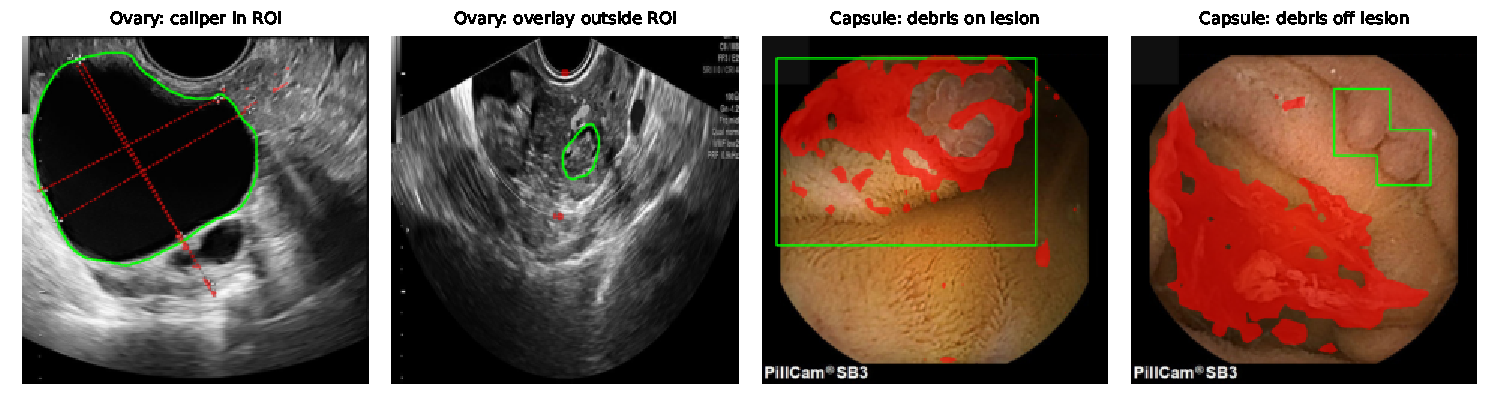
\includegraphics[width=\textwidth]{figures/examples.pdf}
\caption{Real in-ROI and out-of-ROI artifacts (openly licensed cohorts). Green: ROI; red: artifact mask. Left: MMOTU
ovarian tumours (caliper inside the tumour; overlay outside). Right: SEE-AI capsule frames (debris on and off the
lesion box).}\label{fig:examples}\end{figure*}
\fi
